\documentclass{exam}
\usepackage{graphicx} % Required for inserting images
\usepackage[margin=1in]{geometry}
\usepackage{amsmath}
\usepackage{amssymb}
\usepackage{listings}
\usepackage{gfsartemisia-euler} % best font in da game
\usepackage{float}
\usepackage{tikz}

\title{Midterm Exam}
\author{ECE 5/6930 - 004}
\date{October 3, 2025}

\begin{document}
\begin{flushright}
Chandler Justice - A02313187
\end{flushright}
\textbf{ST: Reinforcement Learning} - Midterm Exam\\
\textbf{Due:} October 6, 2025 @ 08:30\\

\noindent \underline{\hspace{3in}}\\


\section{Multiple-Choice}

\textbf{Explain why the correct answer is the correct answer since we gave you the answers}

\begin{enumerate}
    \item What is the difference between on-policy and off-policy algorithms?         
        \begin{enumerate}
            \item On-policy algorithms use a single policy for both acting and learning, while off-policy algorithms use a target policy for acting and a behavioral policy for learning from rewards. (Correct)\\
                \textit{The correct policy approach depends on the application, but a primary advantage of an off-policy is the ability to decouple learning the optimal policy from the policy currently being acted on. In our first homework, we learned a policy from observing a random actor, but by observing this actor we were able to create a policy that when deployed as the actor was much more proficient at the task. Off-policy learning also has the advantage of not being as susceptible to converging into a local minima as the behavior can differ from the greedy policy target. In some applications it may make more sense to use an on-policy technique, such as training a robot to walk using real hardware.}
            \item On-policy algorithms use deterministic policies while off-policy algorithms use stochastic polices.
            \item On-policy algorithms choose the best action without any exploration. Off-policy algorithms chooses the best action with exploration.
            \item On-policy algorithms uses models to learn while off-policy algorithms don't.
        \end{enumerate}
    \item What are the inputs and output of the State Value Function?
        \begin{enumerate}
            \item Inputs: Current state, Output: Expected total reward (Correct)\\
            \textit{The reason we use the current state is because in the State Value Function we assume
            the environment has the Markcov property which means the future only depends on the present, so we only need the current state to determine the value of the state we are in. We output the expected total reward as the value function is meant to provide insight on the long-horizon impact of the current state, providing context where the immediate reward value might be misleading.}
            \item Inputs: Next state, chosen action Output: Expected immediate reward
            \item Inputs: Reward of current state Output: Proposed action
            \item Inputs: Next State Output: Updated policy
        \end{enumerate}
    \item In a MDP, what is the separation between agent and environment?
        \begin{enumerate}
            \item The environment is everything that the agent can not control. (Correct)\\
                \textit{This is important for correctly formulating the control mechanisms available to the agent. While the battery powering the computer the agent is running on might semantically be a part of the agent, making the battery a part of the environment is the correct decision as the agent cannot manipulate the current charge of the battery.}
            \item The environment chooses the actions and the agent records the rewards.
            \item The agent can control the environment and the environment provides feedback.
            \item There is no real separation between environment and agent.
        \end{enumerate}
    \item In DQN, what is the role of the replay buffer?
        \begin{enumerate}
            \item To break correlation by randomly sampling from the agent's past experiences stored in the buffer. (Correct)\\
            \textit{The replay buffer stores experiences $(s, a, r, s')$ and allows random sampling during training. A key advantage of the replay buffer is it prevents the agent from falling into a local minima. If an agent falls into a certain traversal path through greedy traversal of states this can result in a sub-optimal policy. Using the replay buffer can diminish this effect as it adjusts the policy with regards to the experiences sampled. Additionally, this can result in faster convergence as the past experiences are reinforced multiple times over meaning less samples are needed overall.}
            \item The time it takes for an agent to analyze what the best action would be in a state
            \item Used to store only high-reward actions
            \item Computes the reward signal for each action
        \end{enumerate}
    \item With a Q-Learning, how can we guarantee that we will converge on an optimal solution (assuming a proper decaying step-sized is used)?
        \begin{enumerate}
            \item As long as every state-action pair is continually updated then you will converge. (Correct)\\
                \textit{Analytical proofs for this claim are not provided in the textbook; however, there are many properties which Q-learning possess which imply convergence under specific conditions. Specifically}
            \begin{itemize}
                \item \textit{Every state-action pair is visited infinitely often (in implementation this means enough for 'sufficient' exploration)}
                \item \textit{Q-Learning is an off-policy TD control method}
                \item \textit{Q-Learning is applied to an environment with finite states and actions. (Note: most proofs make this assumption, but some literature has shown that Q-learning can converge in continuous cases)}
                \item \textit{Rewards are bounded ($r_t \neq \infty$ as $t \to \infty$)}
            \end{itemize}
            \item Always choosing the action that yields the highest reward will guarantee convergence.
            \item Setting $\gamma = 1$ will cause convergence.
            \item The Q-values should always be increasing to cause convergence.
        \end{enumerate}
\end{enumerate}


\section{Short Response}
\begin{enumerate}
    \item Explain how the Action-Value Function works. Write the Bellman equation and explain each component.
    
        \textbf{Solution:} The bellman \textit{expectation} equation states
    \begin{align*}
        q(s,a) &= \mathbb{E}_{\pi} \left[G_t | S_t = s, A_t = a \right]\\
               &= \sum_{s', r} p(s', r| s, a) \left[r + \gamma \sum_{a'} \pi(a'|s') q_{\pi}(s',a')\right]
    \end{align*}
    Lets go through what each component of this equation is doing:
    \begin{itemize}
        \item $p(s', r| s, a)$: This gives us the probability of getting a reward in a future state $s'$ from our current state. When we take the sum of all of these values they will add up to 1, meaning we are exploring all possible future states
        \item $\left[r + \gamma \sum_{a'} \pi(a'|s') q_{\pi}(s',a')\right]$: This gives us the expected future value given all possible future actions and states, and our current policy. 
    \end{itemize}
    
    The allows us to get a long-horizon outlook on the quality of a state action pair. When we are picking an action, there may be a choice which looks optimal from a greedy perspective, but which actually only leads to a locally optimal solution, meaning we converge to a sub-optimal policy. By evaluating the long-term quality of a state-action pair, we can pick an action which immediately gives a lower reward, but in the long term will result in a higher value overall.

    \item How does the Q-Table relate to the Action-Value function in Question 1?\\
        \textbf{Solution:} The Q-Table relates a given state and action and provides the expected cumulative discounted return given the pair. The entries in the Q-table are updated with
        \[Q(s,a) \leftarrow Q(s,a) + \alpha \left[r + \gamma \underset{a'}{\text{max}}Q(s',a') - Q(s,a) \right]\]
        When an action and reward is visited, the entry in the Q-Table is updated to reflect the reward obtained, plus the estimated value of taking optimal future values. As time increases, the Q-table will converge towards the true action-value function. This provides a significant computational advantage over directly computing the action-value function.
        
    \item How does DQN differ from Q-Learning? What are some improvements that DQN brings?\\
        \textbf{Solution:} DQN utilizes a neural network instead of using a Q-table. This allows for utilizing the same principals of Q-learning without having to keep a tabulation of all possible key-value pairs, which in turn means this learning technique can be applied to much larger environments. Additionally, DQN provides a replay buffer which randomly samples the environment allowing for faster convergence to an optimal policy alongside breaking up breaking up correlations which can arise when following sequential state-action pairs.\\

        Another key distinction is the target network which provides additional stability through less frequent updates versus the main Q-network. These less frequent updates stabilize training which can arise from the constant change in target values.
\end{enumerate}
\newpage
\section{Q-Table by Hand}
You get to generate by hand what the Q-Table representation of this gridworld is going to be! Recall that the formula for updating your Q-Table is:
\begin{equation*}
    Q(s,a) = Q(s,a) + \alpha(r + \gamma \max_{a'}(Q(s',a')) - Q(s,a))
\end{equation*}
Where $a \in A, A = \{Up, Down, Right, Left\}$ and $s \in S, S = \{S_0, S_1, S_2, S_3\}$
Assume $\alpha = 0.5$ and $\gamma = 1.0$

(For every action taken, assume 0 reward if not in a terminal condition.)
Please compute 5 iterations of the Q-table as it learns.

\begin{figure}[h]
\centering
\resizebox{0.30\textwidth}{!}{
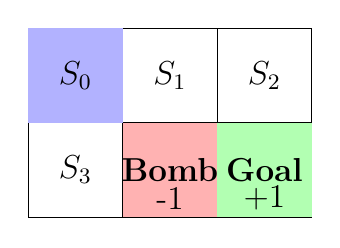
\begin{tikzpicture}[scale=1.2, every node/.style={font=\large}] % larger font
  % Draw 2x3 grid (x=columns, y=rows)
  \draw[step=1,black,thin] (0,0) grid (3,2);

  % Highlight cells
  \fill[blue!30] (0,1) rectangle (1,2);   % Start (S_0)
  \fill[red!30]   (1,0) rectangle (2,1);   % Bomb
  \fill[green!30]  (2,0) rectangle (3,1);   % Goal

  % Top row states
  \node at (0.5,1.5) {$S_0$};
  \node at (1.5,1.5) {$S_1$};
  \node at (2.5,1.5) {$S_2$};

  % Bottom row
  \node at (0.5,0.5) {$S_3$};
  \node at (1.5,0.5) {\textbf{Bomb}};
  \node at (1.5,0.2) {-1}; % Reward under Bomb
  \node at (2.5,0.5) {\textbf{Goal}};
  \node at (2.5,0.2) {+1}; % Reward under Goal
\end{tikzpicture}
} % end resizebox
% \caption{}
\end{figure}

We have provided for you what you should get on the second iteration:  

\begin{table}[H] % use [H] if you want it exactly "here" (requires \usepackage{float})
\centering
\begin{tabular}{c|c|c|c|c}
\textbf{State} & \textbf{Up} & \textbf{Down} & \textbf{Left} & \textbf{Right} \\
\hline
S$_0$ & 0      & 0     & 0     & 0 \\
S$_1$ & 0      & -0.75 & 0     & 0.25 \\
S$_2$ & 0      & 0.75  & 0.125 & 0 \\
S$_3$ & 0      & 0     & 0     & -0.75 \\
\end{tabular}
\caption{Iteration 2}
\end{table}

\section{Graduate Students: Probabilistic Q-Table by Hand}

Please add two complexities to this problem:

\begin{itemize}
    \item Teleportation on wall hit: whenever you hit a "wall" or edge of the gridworld, you have an equal chance to randomly teleport to any of the six cells
    \item Random motion: On moving, every action has a $20\%$ chance of randomly picking a direction to move
\end{itemize}

You are welcome to either take the expectations/probabilities directly or emulate with a random number.

Compare the above with a situation where you have an action cost (for each action taken) of $-0.25$, and comment on the changes in the Q table?

\end{document}
